\section{Comparing Exclusion Limits between ML Models and Previous Analysis}
In the previous section I compared the achieved significance between 
the three optimal models for the full statistics signal set. In this section 
I will do the same, but with the introduction of a flat uncertainty in the background.
Additionally, I will compare the achieved exclusion limits (the mass combinations with an achieved 
significance of over 1.64) by the models created in this thesis, with the limit set in the paper by ATLAS 
in 2021 \cite{atlas_search_2021}.
\\
In the analysis by ATLAS, they have not assumed a flat uncertainty. Instead, an analysis has been made based on 
individual regions and collision processes. Due to time constraints, a flat uncertainty has been made for comparison 
reasons. Aligning with what I have found when reading similar analysis (as well as based on recommendation from my supervisors), 
the uncertainty will be in the region of $20\%$ of the \ac{SM} background. To further study the limits, I will additionally 
compare the models with an uncertainty of $10\%$.\\
\begin{figure}
    \makebox[\linewidth][c]{%
    \centering
    \begin{subfigure}{.75\textwidth}
        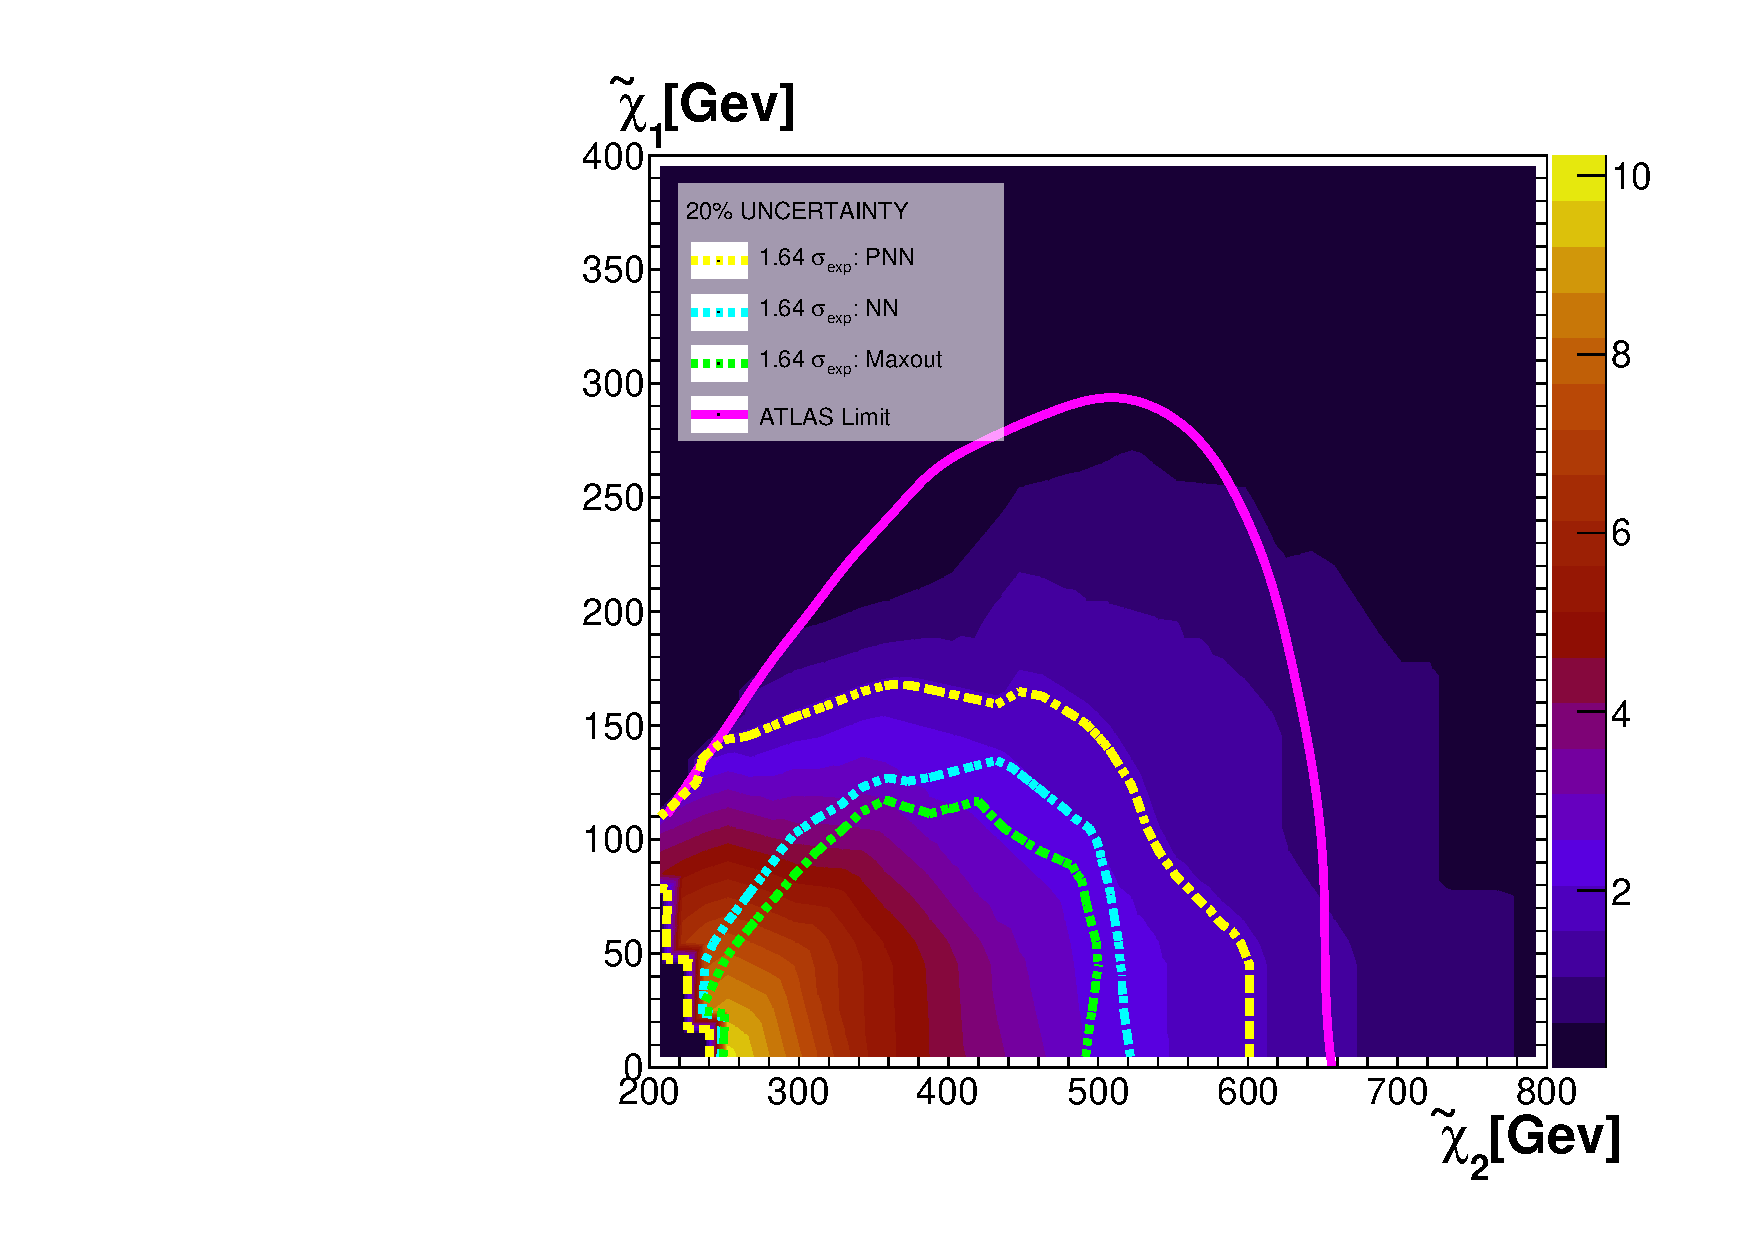
\includegraphics[width=\textwidth]{Figures/MLResults/NN/SUSY/Comparison/Limits/compLimit20.pdf}
    \end{subfigure}
    }
    \caption{A surface plot of the significance achieved by the \ac{PNN} on the full statistics signal set. Contours are 
    drawn around the band equal to a significance of 1.64 for the \ac{PNN} (yellow), dense \ac{NN} (cyan), maxout model (green)
    and the ATLAS analysis (pink). The significance achieved by the \ac{ML} models were calculated with a flat uncertainty equal 
    to $20\%$ of the background.}
    \label{fig:compLimit20}
\end{figure}
In figure \ref{fig:compLimit20}, I have drawn the contours of the significance achieved using the \ac{PNN},
while outlining all points corresponding to a significance of 1.64. The same outline has been made on top of the 
contours of the \ac{PNN} for the dense \ac{NN}, maxout model and the statistical analysis made by ATLAS. The calculations
of the significance for the output of the \ac{ML} models were made with a flat uncertainty equal to $20\%$ of the background.
The figure shows that none of the models are able to extend the sensitivity achieved by ATLAS, although the \ac{PNN} was able to equal
the ATLAS analysis for smaller masses.
\\
A similar figure to what was presented above, was made in figure \ref{fig:compLimit10}. This figure presents the results while applying an
uncertainty equal to $10\%$ of the background. Compared to the limits in figure \ref{fig:compLimit20}, figure \ref{fig:compLimit10} displays 
a far closer comparison between all three models and the results from ATLAS. In this comparison, the dense \ac{NN} and maxout model were able 
to extend the sensitivity of the \ac{PNN} for larger masses of both $\tilde{\chi}_1$ and $\tilde{\chi}_2$, but were beaten in most areas. The 
\ac{PNN} is very close to being able to extend the sensitivity from ATLAS, for high masses of $\tilde{\chi}_2$ and low masses of $\tilde{\chi}_1$. 
\begin{figure}
    \makebox[1\linewidth][c]{%
    \centering
    \begin{subfigure}{.6\textwidth}
        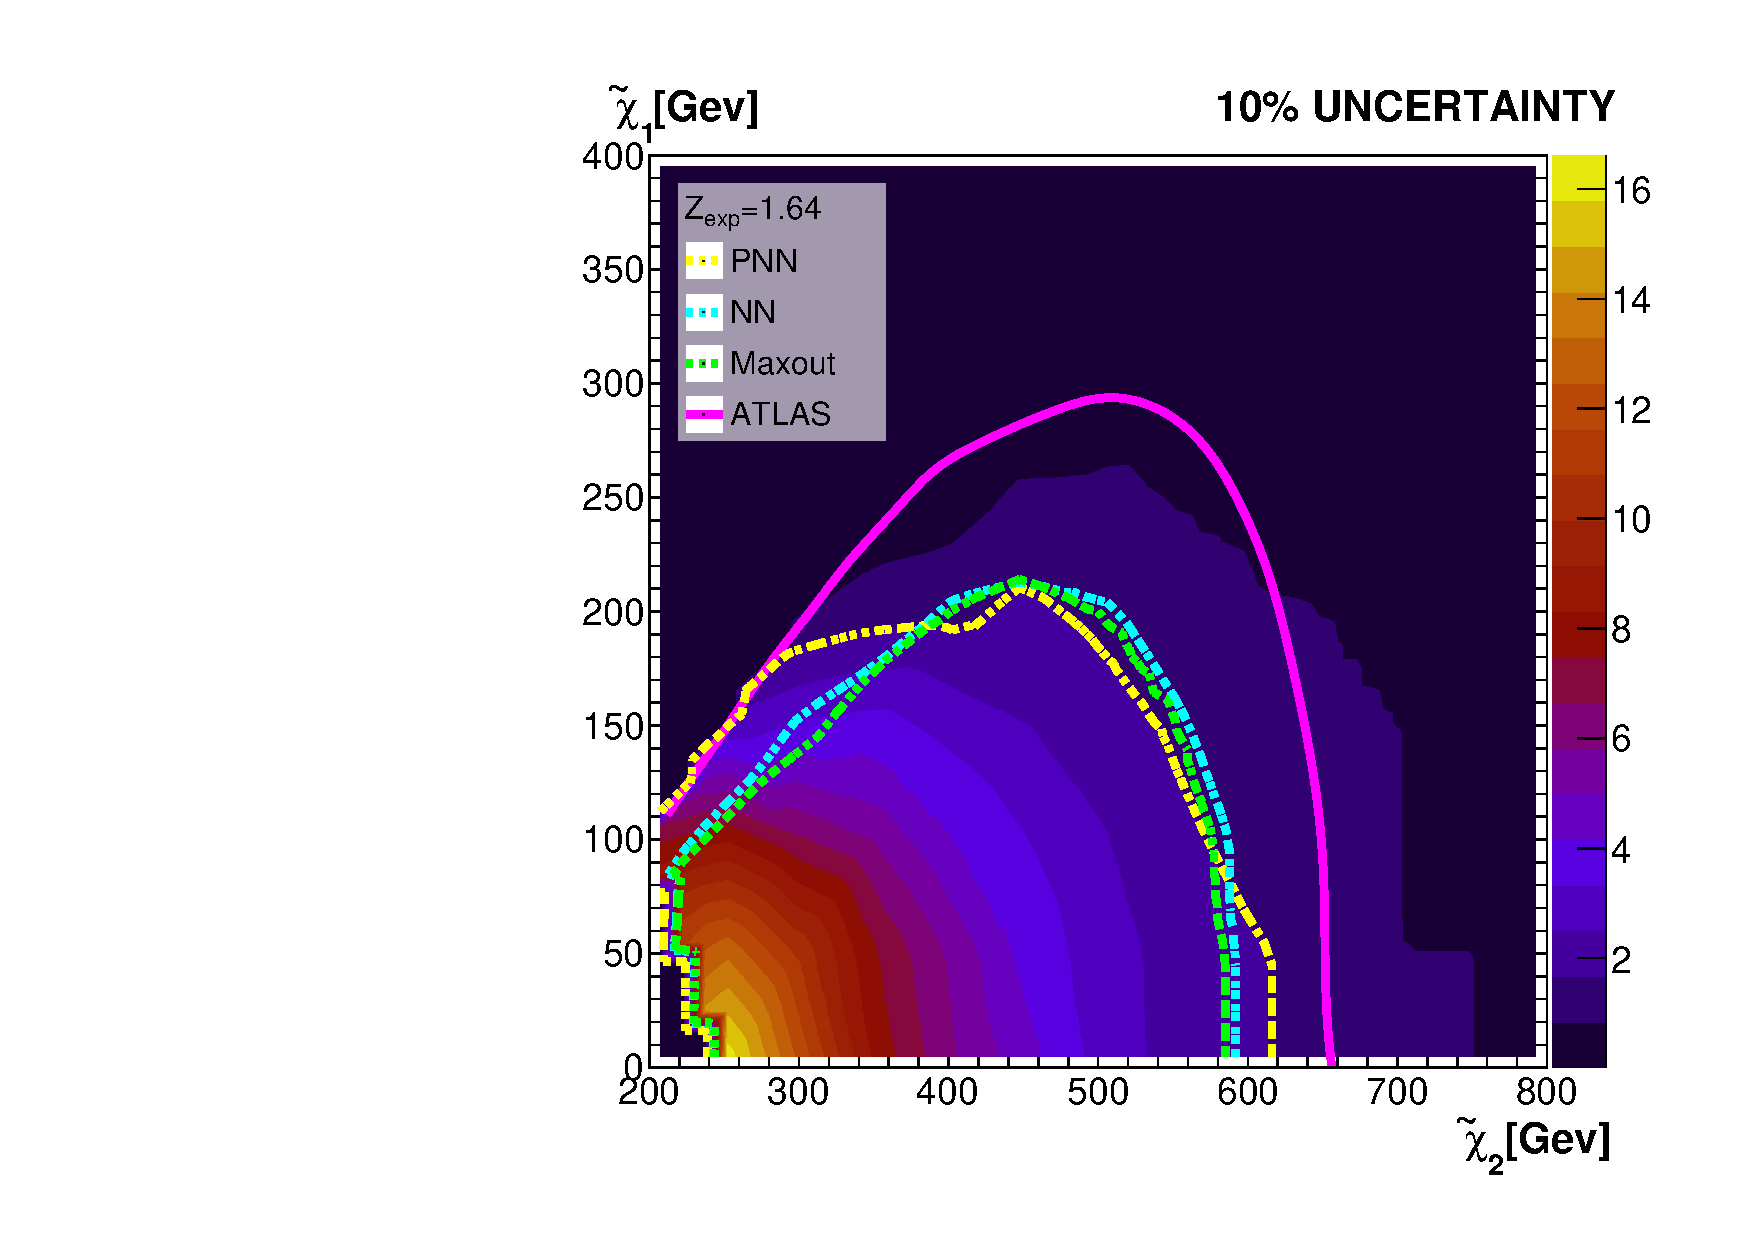
\includegraphics[width=\textwidth]{Figures/MLResults/NN/SUSY/Comparison/Limits/compLimit10.pdf}
        \vspace{-1.cm}
        \caption{}
        \label{fig:compLimit10}
    \end{subfigure}
    \begin{subfigure}{.6\textwidth}
        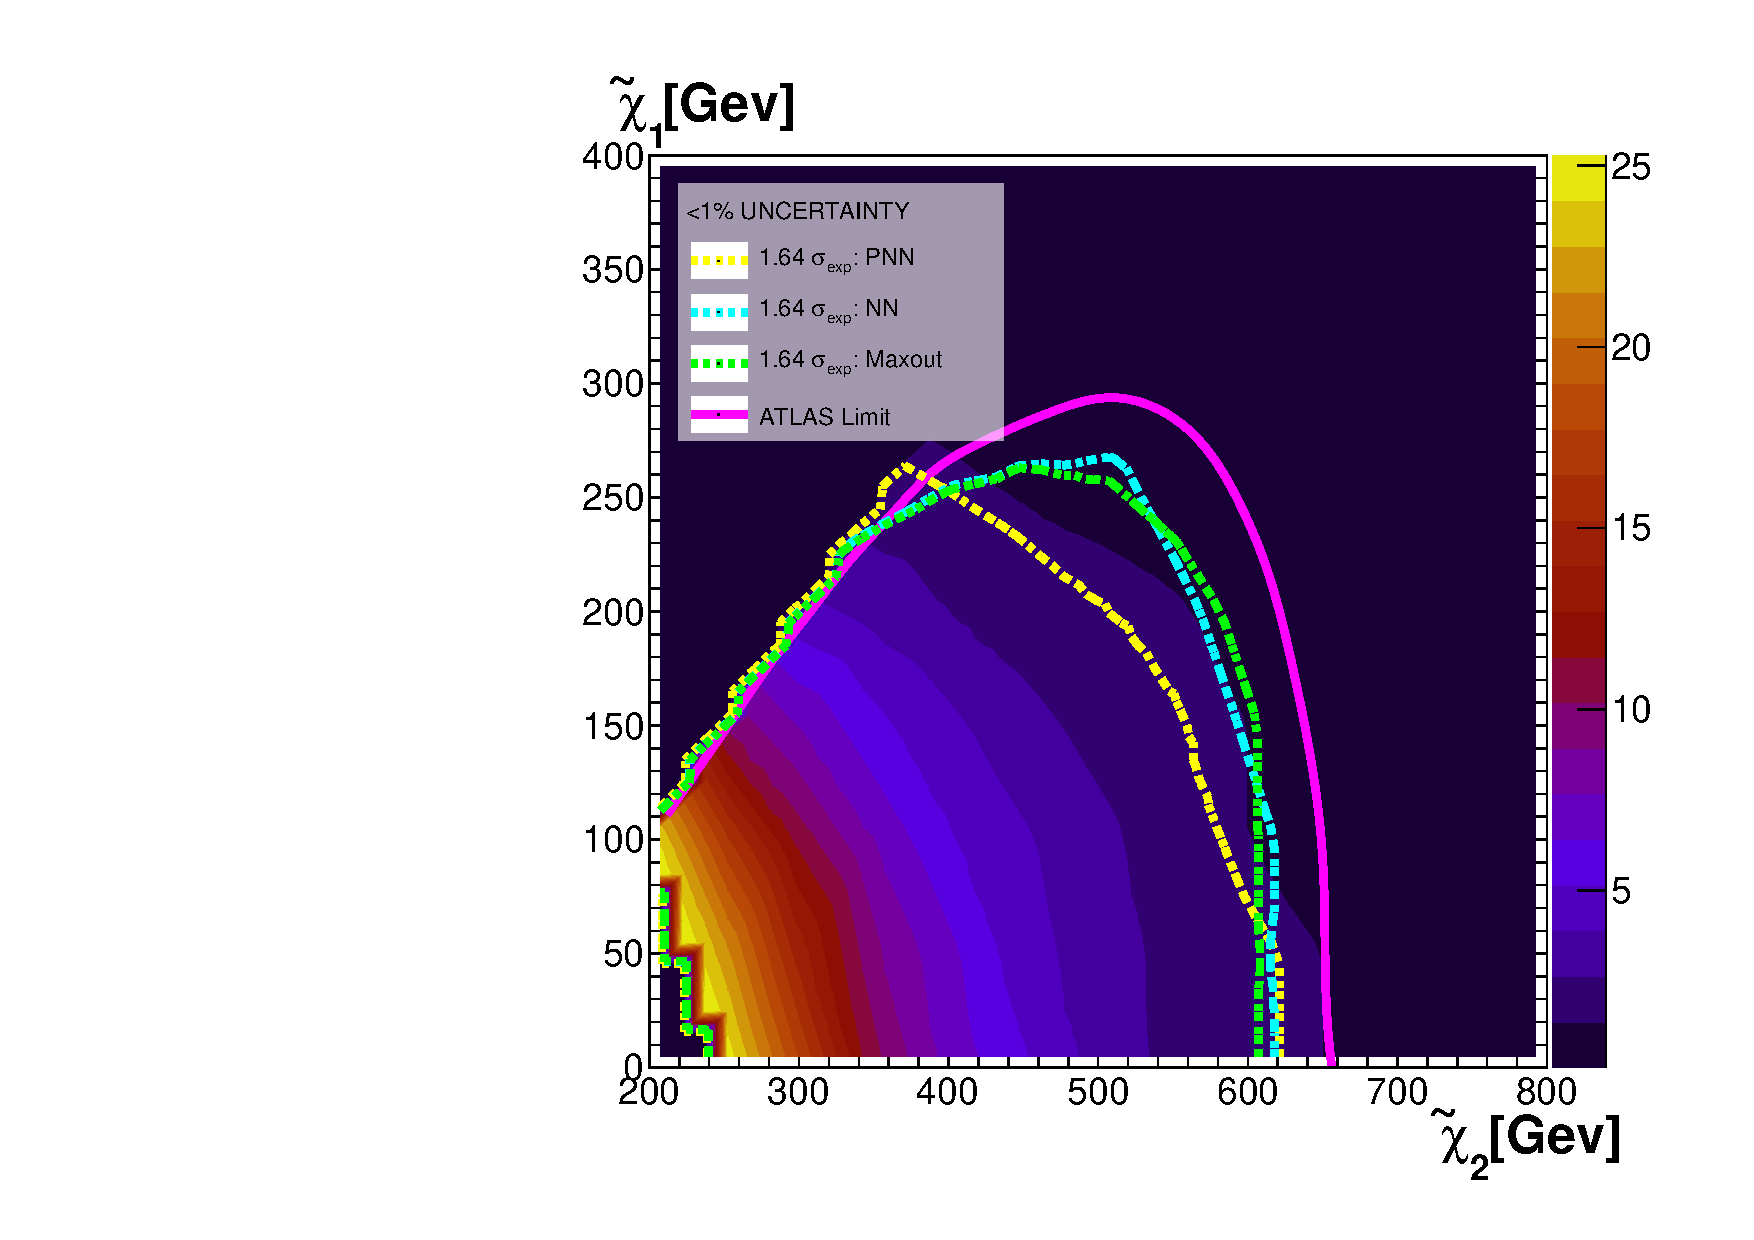
\includegraphics[width=\textwidth]{Figures/MLResults/NN/SUSY/Comparison/Limits/compLimit1.pdf}
        \vspace{-1.cm}
        \caption{}
        \label{fig:compLimit1}
    \end{subfigure}
    }
    \caption{Two surface plots of the significance achieved by the \ac{PNN} on the full statistics signal set. Contours are 
    drawn around the band equal to a significance of 1.64 for the \ac{PNN} (yellow), dense \ac{NN} (cyan), maxout model (green)
    and the ATLAS analysis (pink). The significance achieved by the \ac{ML} models were calculated with a flat uncertainty equal 
    to $10\%$ of the background in the left figure \ref{fig:compLimit10} and less than $1\%$ in the right \ref{fig:compLimit1}.}
\end{figure}